\documentclass[11pt]{article}

\usepackage{fullpage}
\usepackage{graphicx}

\begin{document}

\title{ARM Checkpoint}
\author{A. Spina, E. Rossi, T. Tenev, K. Ciszek}

\maketitle

\section{Group Organisation}

We decided that all team members should work together on each part of the project so that each of us can understand all the tasks and gain as much knowledge as possible on the concepts involved when implementing emulators and assemblers, working with GPIO, etc. For the implementation of Part I a waterfall model was used and all team members contributed. We began by learning the basic principles to get started with programming in C\cite{cbible} before formalising the specification. In order to come up with a design we had to look at \cite{ctopics} and \cite{artandscience} for a good introduction to modular development and compound data types. A more detailed overview of the design is provided in the next section.

The code repository was structured according to \cite{gitmodel} and we adopted a standard convention for commit messages \cite{gitcommit}. Merge requests were used as a fundamental part of the development process. Each merge request was created by one or two team members and the code was reviewed by another member who had not been directly involved in writing it.

Unit testing was encouraged right from the start of implementation and a minimal approach \cite{minunit} was adopted. This enforced the existence of self-contained testable modules. Continuous integration was configured to build the make targets and run all tests on each push to all remote branches.

We will continue applying professional practices to improve the overall structure of the project. The current workflow has produced satisfactory results and can be accelerated as team members become more comfortable with the implementation details.

\section{Implementation Strategies}

\subsection{Emulator design}

The emulator state (memory and registers) is encapsulated in a module which provides an interface for reading and writing words, bytes, and registers. Memory is represented by an array of a union type which is useful for working with different representations of a word (raw binary, separate bytes, or a decoded instruction). Decoded instructions are also represented by a union of bit field structures for each of the 4 formats. Memory is initialised by setting the raw binary field of each word when reading and using the decoded instruction representation through a pipeline module. The pipeline decodes the type of instruction and calls one of 4 specific handlers. The handler interface exposes a single execution function which is polymorphic on the decoded instruction type.  As this is a union type this pointer can be used inside the handlers safely without casting.
A diagram representing the design is shown in Figure \ref{fig:arm11}.

\subsection{Code reusability}

The design can be easily extended to support more instruction types or a more sophisticated pipeline. Moreover, with a clever assembly source tokeniser the memory data structure can be completely reused when implementing the assembler.

In addition to that, we have already set up a testing and a continuous integration framework, so we will be able to keep using those parts in the next stages of the project without having to spend time to set them up again. 

\subsection{Future Challenges}

One of the biggest challenge we are facing is that we are having difficulty coming up with a suitable extension, mainly because of our lack of experience in C and Assembly makes it hard to estimate what we could achieve in the given time. 

At the same time, The Raspberry Pi is a completely new piece of hardware for most of us and we will have to learn the basics before being able to work on the GPIO part. This is why we will concentrate on finishing the assembler before proceeding with the later stages of the project.
We will possibly also struggle when approaching Part 3, as we have had little experience with Assembly during the year.

\medskip

\begin{figure}[h]
\caption{Diagram of emulator design}
\centering
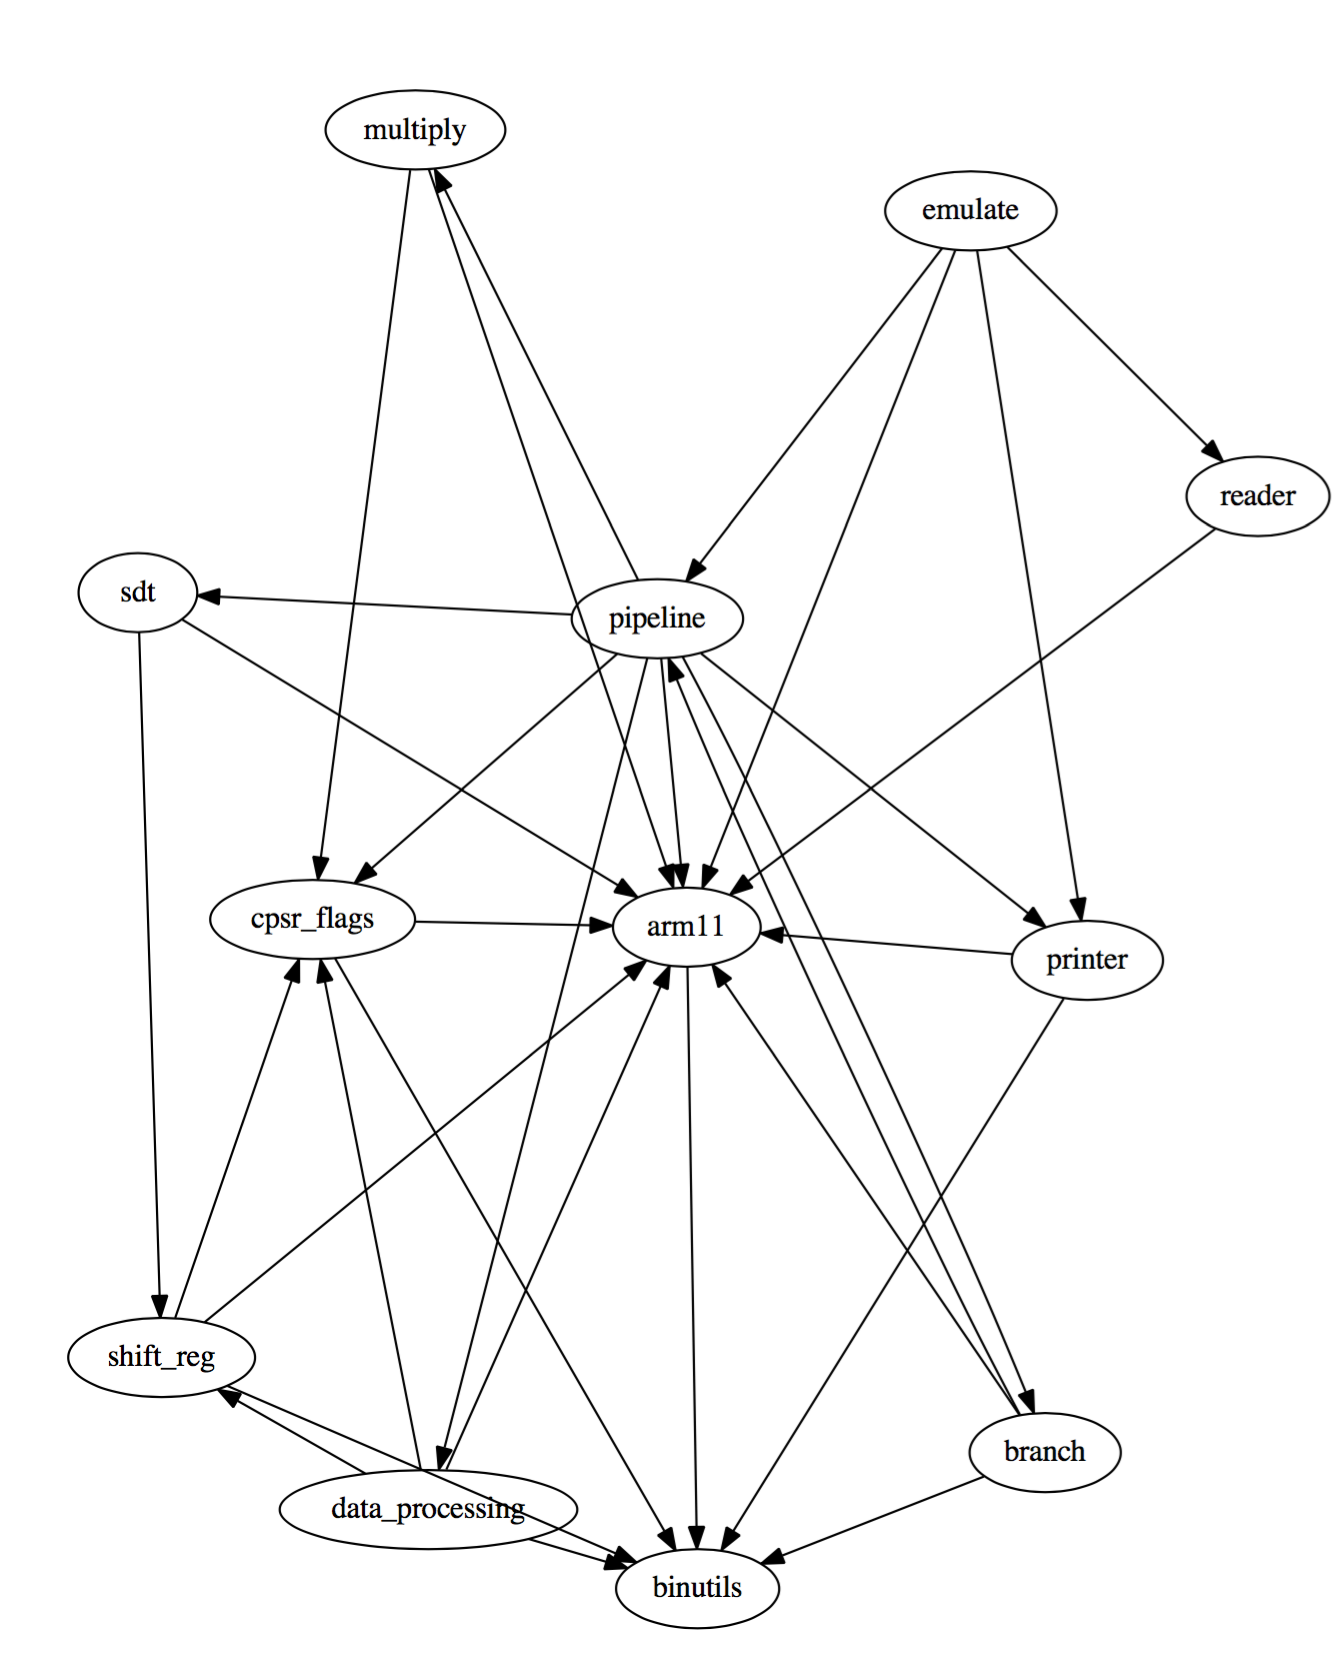
\includegraphics[scale=0.7]{arm11-modules.png}
\label{fig:arm11}
\end{figure}

\begin{thebibliography}{7}

\bibitem{cbible}
Kernighan, B. and Ritchie, D. (1988).
\textit{The C programming language.}
Englewood Cliffs, N.J.: Prentice Hall.

\bibitem{ctopics} 
Kochan, S. and Wood, P. (1987).
\textit{Topics in C programming.}
Indianapolis, Ind., USA: Hayden Books.
 
\bibitem{artandscience} 
Roberts, E. (1995).
\textit{The art and science of C.}
Reading, Mass.: Addison-Wesley Pub. Co.

\bibitem{gitmodel}
Driessen, V.
\textit{http://nvie.com/posts/a-successful-git-branching-model/}

\bibitem{gitcommit}
Beams, C.
\textit{http://chris.beams.io/posts/git-commit/}

\bibitem{minunit}
Brewer, J.
\textit{http://www.jera.com/techinfo/jtns/jtn002.html}

\end{thebibliography}

\end{document}
